% !TEX root = thesis-thomas-tiotto.tex

\section{Methods} 
\subsection{Libraries}
\subsubsection{pomegranate}
\textit{pomegranate} (\cite{pomegranate}) is an open-source probabilistic models package for python.
Its core philosophy is that every probabilistic model, from Hidden Markov to Bayesian Network, can be seen as a probability distribution and, as such, can be flexibly composed into hierarchical mixture models (\cite{Schreiber2017}).
The package implements:
\begin{itemize}
	\item Probability Distributions
	\item General Mixture Models
	\item Hidden Markov Models
	\item Bayes Classifiers and Na{\"i}ve Bayes
	\item Markov Chains
	\item \textbf{Bayesian Networks}
	\item Factor Graphs
\end{itemize} 

This package was chosen among others for its good implementation of Bayesian Networks, its clear API and its performance.
The package is written in cython and natively supports multi-core parallelism and out-of-core learning.
Network structure learning from data, described in \ref{subsec:bnstructurelearning}, appears to be particularly efficient, thanks to the implementation of prior knowledge into the graph selection process as described by \cite{schreiber_noble_2017}.
The claim of this novel selection process is that it possesses the speed of a heuristic approach while yielding a far better quality estimate.

pomegranate currently only supports Discrete Bayesian Networks so the random variable of each node must have a categorical distribution.

\textit{Structure learning} from data is achieved using the \texttt{from\_samples} method of the \texttt{BayesianNetwork} class, with the default algorithm being the novel one described by \cite{schreiber_noble_2017}.
The \textit{probability} of a sample is calculated using the \texttt{probability} function of an object of \texttt{BayesianNetwork} type; the \texttt{predict\_proba} function is used to return the probability of each variable in the model given some evidence.
\textit{Predictions} (described in detail in Sec. \ref{subsec:bnupdating}) are run by passing to the \texttt{predict} function of an object a matrix with \texttt{None} as placeholders for missing values .
\textit{Fitting} is done thought the \texttt{fit} function that uses MLE estimates to update each node's distribution in the model based on the input data.

A \texttt{BayesianNetwork} object can also be displayed graphically by calling its \texttt{plot} function.
The output is a DOT file that is generated using the PyGraphviz package (\cite{pygraphviz}), that is a python interface to the famous Graphviz (\cite{graphviz}) graph visualisation software.
An example of such an output is shown in Fig. \ref{fig:pomegranate_graph_example}.

\begin{figure}[htbp]
\centerline{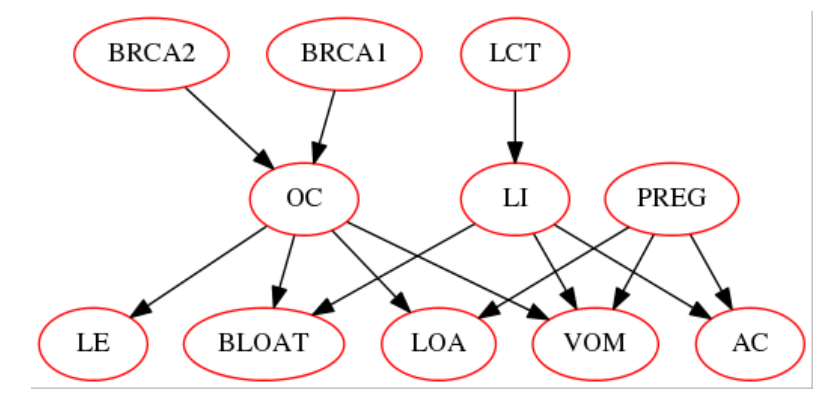
\includegraphics[width=\columnwidth]{methodology/images/pomegranate_example}}
\caption{Example output of \texttt{plot} (\cite{pomegranatetutorial}) }
\label{fig:pomegranate_graph_example}
\end{figure}

\subsubsection{Gurobi}
\textit{Gurobi} (\cite{gurobi}) is a closed-source mathematical programming solver for Linear Programming, Quadratic Programming and Mixed-Integer Programming optimisation problems.
It calims to be the fastest solver available.
Gurobi offers object-oriented and matrix-oriented interfaces to, among others, Python, MATLAB and Excel.

\subsubsection{pandas}
\textit{pandas} (\cite{pandas}) is an extremely widely-used open-source python library that provides data structures and methods to aid in data analysis.
The package excels in the manipulation of tabular data in the form of \texttt{DataFrame}, that is the analogous of R's \texttt{data.frame}.
A \texttt{DataFrame} can be seen as a \enquote{general 2D, size-mutable structure with potentially heterogeneously-typed columns}.
The syntax for slicing is very close to R's as are many other functionalities; this is because one of Pandas' explicit goals is to offer all of CRAN's functionalities and be easily approachable by anyone already knowing the other language.

Pandas the default choice for this thesis' implementation because it is the \textit{de facto} standard in data analysis applications.
Its flexibility in reading Excel spreadsheets (the format the data set the project was built on, see Sec. \ref{sec:data-set}) and in then manipulating the data confirmed that this was a good choice.
Note that to read files in the Excel formats the additional \texttt{xlrd} package is needed.

\subsubsection{scikit-learn}
\textit{scikit-learn} (\cite{scikitlearn}) aims at providing a unified API for basic Machine Learning; it does not include advanced paradigms such as Reinforcement Learning or graphical models for structured learning.
The latter omission was the reason that lead me to select pomegranate as the basis for the implementation of a Bayesian Network.
What is included are a stack supervised and unsupervised ML tools to prepare data sets, define machine learning models ranging from spectral analysis-based to ensemble methods to clustering and multiple evaluation and model selection utilities.

\subsubsection{NumPy}
\textit{NumPy} (\cite{numpy}) is another \textit{de facto} standard package when doing scientific computing with python.
Most scientific packages (including pandas, scikit-learn and TensorFlow) depend on NumPy for low-level operations; this is because NumPy is contains fast implementation of n-dimensional array objects together with powerful manipulation functions.
In addition to this, NumPy implements linear algebra operations, Fourier Transform and random number generation.
The closest parallel to NumPy - as R was for pandas, is MATLAB.

\subsubsection{networkx}
\textit{NetworkX} (\cite{networkx}) is another widely-used package that is specialised in the creation and manipulation of graph-structured data.

\subsubsection{anytree}
\textit{anytree} (\cite{anytree}) is a python package giving a lightweight implementation of a tree data structure and traversal methods.


\subsection{Algorithms}
\subsubsection{d-separation}
A na{\"i}ve implementation according to the definition (presented in Subsec. \ref{subsec:bayesiannetworks}) to check for d-separation between node $X$ and $Y$ would have a complexity in the order of the number of trails between $X$ and $Y$; this leads to an exponential in the size of the graph running time.
Luckily, \cite{koller2007dseparation} present what is a linear time algorithm to solve the problem.

The \texttt{reachable} procedure takes as input the DAG representing the Bayesian Network $\mathcal{G}$, a source variable $X$ and a set of observed variables $Z$; on exit it returns the set of variables $R$ that are reachable from $X$.
The procedure runs in two phases, traversing the graph twice: first bottom-up from leaves to roots, then viceversa.
During the first run, the algorithm finds all nodes $A$ that are ancestors of the evidence set $Z$.
During the second, the procedure distinguishes the direction it visits each node in order to determine if it is traversable or not.
Any node $Y$ that is not in the evidence set is marked as reachable; if it is being visited in direction \enquote{up} it can be traversed as the v-structure is a chain.
All the parents of $Y$ are marked to be visited in the \enquote{up} direction (i.e. from below) and the converse is done for $Y$'s children.
If $Y$ is being visited in the \enquote{down} direction its children are again added to be visited in the \enquote{down} direction, because $Y$ is traversable.
Additionally, if $Y$ happened to be in the set $A$, found in the first step, then $Y$'s parents are marked to be visited in the \enquote{up} direction then the collider is active and $Y$ can be traversed (a collider is open iff. the central node or any of its descendants are observed).

The full procedure can be found in \cite{koller2007dseparation}; my implementation follows this pseudocode very closely but instead of finding all nodes $R$ that are d-connected to the input $X$, tests if a given target $Y$ is d-separated from $X$ or not.
This gives some extra flexibility in how the function can be used.
To find the set $S$ of all nodes d-separated from $X$ I simply iterate the test over all nodes in the graph.
 
\lstset{language=algebra,linewidth=0.95\linewidth,breaklines=true,numbers=left,
basicstyle=\ttfamily,numberstyle=\tiny,escapeinside={//*}{\^^M},
mathescape=true}
\begin{lstlisting}
source // source variable
evidence // evidence set
foreach target in $V$ // $V$ set of variables of the graph
	separated_from_source[target] = d_separated(source,target) // true or false for each variable
\end{lstlisting}


\subsubsection{MPE}
\todo{descrivere come ottenere MPE con Gurobi: exporter, UAI ecc...}
